%%%%%%%%%%%%%%%%%%%%%%%%%%%%%%%%%%%%%%%%%%%%%%%%%%%%%%%%%%%%%%%%%%%%%%%
%%%%%%%%%%%%%%%%%%%%%%%%%%%%%%%%%%%%%%%%%%%%%%%%%%%%%%%%%%%%%%%%%%%%%%%
%%%%%                                                                 %
%%%%%     <file_name>.tex                                             %
%%%%%                                                                 %
%%%%% Author:      <author>                                           %
%%%%% Created:     <date>                                             %
%%%%% Description: <description>                                      %
%%%%%                                                                 %
%%%%%%%%%%%%%%%%%%%%%%%%%%%%%%%%%%%%%%%%%%%%%%%%%%%%%%%%%%%%%%%%%%%%%%%
%%%%%%%%%%%%%%%%%%%%%%%%%%%%%%%%%%%%%%%%%%%%%%%%%%%%%%%%%%%%%%%%%%%%%%%

\chapter{Design Implementation}


\section { Porting Halide to new targets}
    Halide programs relies on the \gls{llvm} libraries to compile code for the desired targets. To build the Halide library, we first need to build \gls{llvm} with the correct flags and add the support for the building machine.
    As the \gls{hero} toolchain already has a build of this compiler, we can use it to compile Halide, but the \texttt{-DBUILD\_SHARED\_LIBS} flag has to be disabled, as Halide does not support shared libraries.
    We added a \texttt{make} target to main \texttt{Makefile} of the project, to simplify the installation process.

    Once the installation process was complete, we worked on porting Halide to \gls{hero} on the hardware simulation. This was the first step of the project, as this platform is easier to work with than the full \gls{hero} platform. We do not have to work with the heterogeneous toolchain, so the compilation process is simpler.
    Unlike the hardware platform, the hardware simulator only simulate a single  \gls{pulp} cluster configured with eight cores.
    The first core of the cluster acts as the host, it first initializes the cluster and then starts the execution of the application.
     When a fork is executed on the other cores, the host core continues the execution like the other cores.
     

    %%%%%%%%%%%%%
    \section{Compilation Workflow}

\begin{figure}[H]
\dirtree{%
    .1 halide-examples/.
    .2 common/.
    .3 defaultHalide.mk.
    .2 myApp/.
    .3 main.c.
    .3 Makefile.
    .3 lib/.
    .4 halidePipeline.cpp.
    }
    \caption{Directory structure for Halide applications.}
    \label{Fig:DirectoryStructure}
\end{figure}



    Every application follows the directory structure described in Figure~\ref{Fig:DirectoryStructure}, the \texttt{common} folder is shared between all the applications and contains a common \texttt{Makefile} that will be included in every application's \texttt{Makefile}.
    The source code is split between two files, the pipeline generator in the \texttt{lib/} folder, and the main \gls{hero} application.
    The pipeline generator uses Halide to generate the pipeline object file which will be linked during the compilation of the application.

\begin{figure}[h]
    \centering
    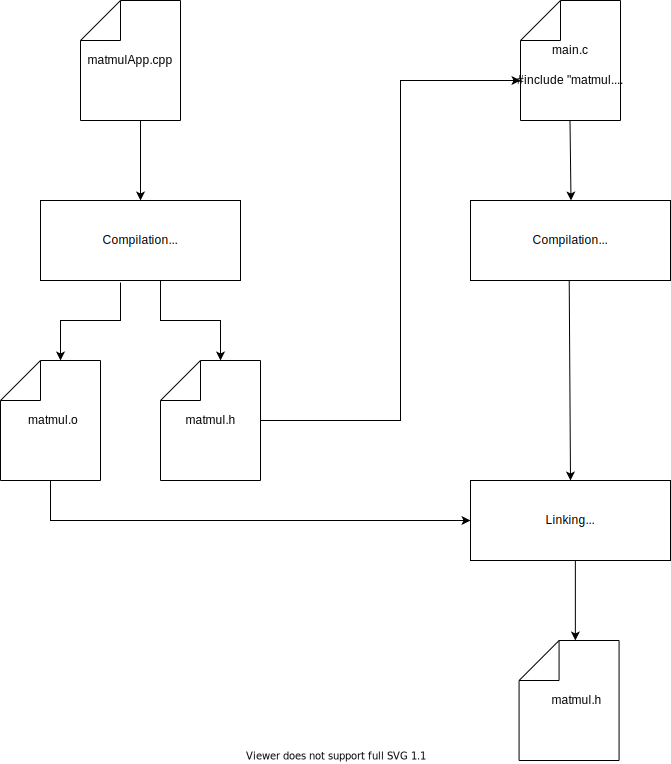
\includegraphics[width=.7\textwidth]{./figures_raw/compilationWorkflow.png}
    \caption{Compilation Workflow for an Halide Application.}
    \label{fig:compwork}
\end{figure}

    Figure~\ref{fig:compwork} shows the whole compilation process to build a Halide application for \gls{hero}.
    The compilation is done in two steps. First, we compile the Halide program to execute on the build computer.
    This program is then run on the machine and creates a RISC-V object file and a header file.
    This header file must be included in the \gls{hero} application (\texttt{main.c}).
    The application building process is based on the \gls{openmp} workflow, we used the same \texttt{Makefile} with some modification to link the pipeline with the main application. 

    We first compile the source code to \gls{llvm} assembly code. Then due to the heterogeneous nature of the system, a custom program: \texttt{hc-omp-pass}, changes every part of the code that may cause issue due to architectural differences between the host and the \gls{pcma} (on \gls{hero}v3, the host can be a 64-bit RISC-V or an ARM processor, and the pointers have to be changed due to the incompatibilities between the 32-bit and 64-bit addressing).
    In our case, as we only compile for the \gls{pulp} cluster, this step does not affect the code, but it will be useful to support the full \gls{hero} platform. 
    Then, we use the \gls{llvm} assembly files coupled with the pipeline object file to generate the final binary.


    The header file generated by Halide declares every function available on Halide and required to have a fully working Halide implementation. 
    Most of them do not use platform-specific functionalities, and will be compiled to RISC-V without any issue.
    But others such as memory management functions or thread distribution functions, which require dedicated functions in the \gls{pulp} runtime have to be overwritten to work on the cluster.
    Finally, functions that are only called when using the Just in Time compilation or other advanced functionalities, have to be overwritten, but we can implement simple stub functions to prevent linking errors, as we do not need those functionalities for our pipelines. 
    The comments in the header precisely describes the role of each function and under which circumstances they have to be overwritten.
    We implemented the necessary functions in the \gls{pulp} runtime to make the parallel schedule work, as this schedule is essential to take advantage of the high core count of the cluster.
 
\section{Schedule Implementation }
    Most schedules work out of the box, because they do not need to access any runtime specific function.
    Halide generates them by altering the source code as operations such as splitting and unrolling are just modification of the loops of the pipeline. 
    Even the vectorize schedule does not need any specific instructions, Halide will rewrite the schedule as if the pipeline was manipulating a vector even if the hardware target does not support \gls{simd} instructions.
     To use this schedule fully,  a hardware specific modification would be needed.
    Memory access and thread task distribution on the cluster have to be overwritten as they use specific runtime functions.

    \subsection{Modification to the PULP runtime}

    The missing Halide functions need to be accessible to the \gls{pulp} runtime. To do so, we created a new file in the \gls{pulp} runtime (\texttt{halide\_api.c}). 
    This file contains all the \gls{api} functions required to run Halide on \gls{hero}.

\begin{lstlisting}[language=C,caption={The \texttt{halide\_do\_par\_for} function.},label={lst:halidedoparfor},captionpos=b]
int halide_do_par_for(void *user_context,halide_task_t task,
    int min, int size, uint8_t *closure) {
    // Mount the cluster
    rt_cluster_mount(1, 0, 0, NULL);

    unsigned arguments[4];
    arguments[0] = (unsigned)user_context;
    arguments[1] = (unsigned)size;
    arguments[2] = (unsigned)closure;
    arguments[3] = (unsigned)task;

    // Dispatch the task to the cluster
    rt_team_fork(0, pulp_do_halide_par_for_fork, arguments);

    // Unmount the cluster
    rt_cluster_mount(0, 0, 0, NULL);

    return 0;
}
\end{lstlisting}


    The Listing~\ref{lst:halidedoparfor} shows the full source code of the \texttt{halide\_do\_par\_for} function.
    This function is only called once during the execution of a parallel schedule. On the hardware simulator, only the first core of the cluster executes it.
    The \texttt{size} argument of the function determines the number of threads to create, and will be used by the cores to determine which task to execute. 
    This function creates the thread pool for the parallel execution of the pipeline. As \gls{hero} does not have a standard way of managing threads, we had to overwrite this function.
    The \texttt{rt\_cluster\_mount} is called to prepare the cluster before distributing the tasks.
    The \texttt{argument} structure packs all the data about the tasks: the user context,  the number of threads, and the starting point of the execution.
    \texttt{rt\_team\_fork} will then create a team of workers which will all execute the same function: \texttt{halide\_do\_par\_for\_fork}.
    The first argument of \texttt{rt\_team\_fork} indicates how many fork the cluster will do, if it is set to zero, the cluster will reuse the last number of threads (which is by default eight).



\begin{lstlisting}[language=C,caption={The \texttt{halide\_do\_par\_for\_fork} function.},label={lst:halidedoparforfork},captionpos=b]
void pulp_do_halide_par_for_fork(void *arg) {
  unsigned *arguments = (unsigned *)arg;

  void *user_context = (void *)arguments[0];
  unsigned task_num = arguments[1];
  uint8_t *closure = (uint8_t *)arguments[2];
  halide_task_t task = (halide_task_t)arguments[3];

  for (unsigned core_id = rt_core_id(); core_id < task_num; core_id += (int)&__rt_nb_pe) {
    task(user_context, core_id, closure);
  }

}
\end{lstlisting}
    The source code of this function is shown in listing~\ref{lst:halidedoparforfork}, every worker iterates over the task queue, and executes only the task they have been assigned.
    The assignment is done by comparing the task identifier with the worker's core identifier, if \texttt{core\_id = task\_id \% nb\_cores}, then the task will be executed by the worker. 
    Finally, once every worker completes, the cluster is turned off.

%% Pros and cons of such a distribution scheme
    
    This distribution scheme has the advantage of being easy to implement and splitting the task is done in a way that facilitates debugging if needed.
    But, it can't adapt if one core is delayed or its task takes longer to compute.
So if one core has to execute some tasks which are two or three times longer to execute, all the other core will wait for this core to compile.
    It may be interesting to dynamically reschedule the tasks depending on the free cores.

